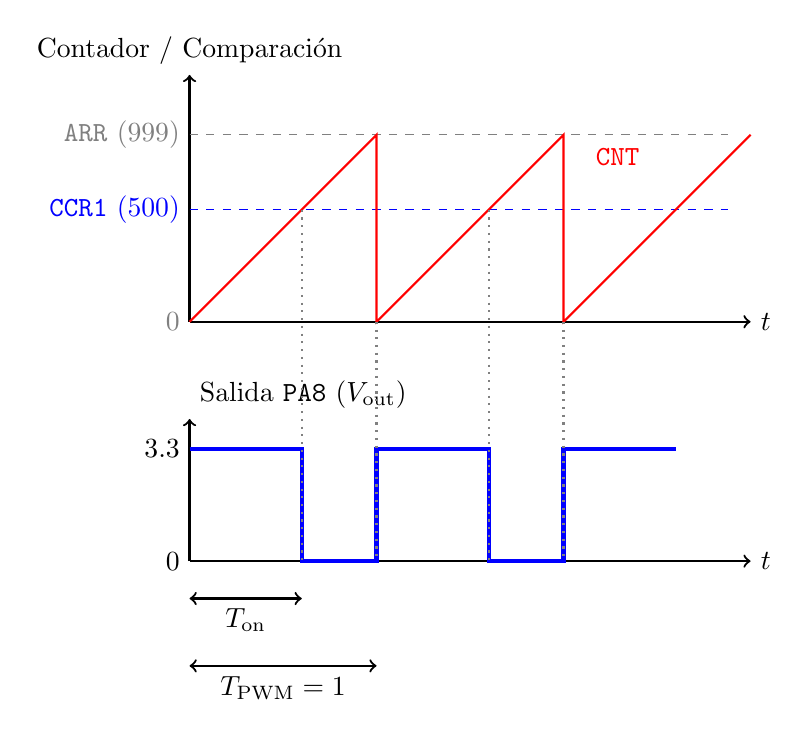
\begin{tikzpicture}[scale=0.95]
  % === SISTEMA SUPERIOR: CONTADOR CNT ===
  \draw[->, thick] (0,0) -- (7.5,0) node[right] {$t$};
  \draw[->, thick] (0,0) -- (0,3.3) node[above] {Contador / Comparación};

  % Niveles de referencia superior
  \draw[dashed, color=gray] (0,2.5) node[left] {\texttt{ARR} (999)} -- (7.2,2.5);
  \draw[dashed, color=blue] (0,1.5) node[left] {\texttt{CCR1} (500)} -- (7.2,1.5);
  \node[left, gray] at (0,0) {$0$};

  % Señal diente de sierra CNT
  \draw[thick, color=red] (0,0) -- (2.5,2.5) -- (2.5,0) -- (5,2.5) -- (5,0) -- (7.5,2.5);
  \node[red, right] at (5.3, 2.2) {\texttt{CNT}};

  % === SISTEMA INFERIOR: SALIDA PA8 ===
  \draw[->, thick] (0,-3.2) -- (7.5,-3.2) node[right] {$t$};
  \draw[->, thick] (0,-3.2) -- (0,-1.3) node[above right] {Salida \texttt{PA8} ($V_{\mathrm{out}}$)};

  % Formación de la onda cuadrada PWM en PA8
  \draw[ultra thick, color=blue] (0,-1.7) -- (1.5,-1.7) -- (1.5,-3.2) -- (2.5,-3.2) -- (2.5,-1.7) -- (4.0,-1.7) -- (4.0,-3.2) -- (5.0,-3.2) -- (5.0,-1.7) -- (6.5,-1.7);

  % Etiquetas de tensión en eje Y inferior
  \node[left] at (0,-1.7) {$\qty{3.3}{\V}$};
  \node[left] at (0,-3.2) {$\qty{0}{\V}$};

  % === LÍNEAS DE PROYECCIÓN VERTICAL ===
  \draw[dotted, thick, color=gray] (1.5,1.5) -- (1.5,-3.2);
  \draw[dotted, thick, color=gray] (2.5,0) -- (2.5,-3.2);
  \draw[dotted, thick, color=gray] (4.0,1.5) -- (4.0,-3.2);
  \draw[dotted, thick, color=gray] (5.0,0) -- (5.0,-3.2);

  % === COTAS TEMPORALES ===
  \draw[<->, thick] (0,-3.7) -- (1.5,-3.7) node[midway, below] {$T_{\mathrm{on}}$};
  \draw[<->, thick] (0,-4.6) -- (2.5,-4.6) node[midway, below] {$T_{\mathrm{PWM}} = \qty{1}{\ms}$};
\end{tikzpicture}
